\chapter{Path Planning for Underwater Robots}
%For path planning with trim trajectory and Frenet-Serret frame, the sway- and heave velocities are always equal to zero. The roll-, pitch and yaw velocities are relatively small with respect to the surge velocity. Thus, we can approximate the velocity of fin relative to the fluid $U_{fin}$ as the surge velocity $u_{fin}$ of the robot. 
% Given the nonlinear system $\dot{\vec{x}}=\vec{f}(\vec{x},\vec{u})$ and a desired trajectory $(\vec{x}_{d},\vec{u}_{d})$. We want to design a controller in the form $\vec{u}=\alpha(\vec{x},\vec{x}_{d},\vec{u}_{d})$ such that $\lim_{t \to \infty}x-x_{d}=0$. Since underwater robots are affine in commanded inputs, the dynamics can be simplified as $\vec{f}(\vec{x},\vec{u})=\vec{f}(\vec{x})+\vec{g}(\vec{x})\vec{u}$. Let us define new error state $\vec{x}-\vec{x}_{d}$ and $\vec{v}=\vec{u}-\vec{u}_{d}$ and we can calculate the error dynamics:
% \begin{align}
% \dot{\vec{e}}=\dot{\vec{x}}-\dot{\vec{x}}_{d}=\vec{f}(\vec{x})+\vec{g}(\vec{x})\vec{u}-\vec{f}(\vec{x}_{d})-\vec{g}(\vec{x}_{d})\vec{u}_{d}
% \\
% =\vec{f}(\vec{e}+\vec{x}_{d})-\vec{f}(\vec{x}_{d})+\vec{g}(\vec{e}+\vec{x}_{d})(\vec{v}+\vec{u}_{d})-\vec{g}(\vec{x}_{d})\vec{u}_{d} 
% \\
% =\vec{F}(\vec{e}+\vec{v},\vec{x}_{d}(t),\vec{u}_{d}(t))
% \end{align}
% For tracking the desired trajectory, we can assume the error $\vec{e}$ is very small if our controller works very well so that we can linearize around $\vec{e}=\vec{0}$: 
% \begin{align}
% \dot{\vec{e}}=\emph{\textbf{A}}(t)\vec{e}+\emph{\textbf{B}}(t)\vec{v}
% \end{align}
%where $ \emph{\textbf{A}}(t)=\dfrac{\partial \vec{F}}{\partial \vec{e}}\Bigr|_{\vec{x}_{d}(t),\vec{u}_{d}(t)} $ and $ \emph{\textbf{B}}(t)=\dfrac{\partial \vec{F}}{\partial \vec{v}}\Bigr|_{\vec{x}_{d}(t),\vec{u}_{d}(t)} $. It is often the case that $\emph{\textbf{A}}$ depend on $ \vec{x}_{d} $. Hence, we can rewrite $ \emph{\textbf{A}}(t)=\emph{\textbf{A}}(\vec{x}_{d})$ and $ \emph{\textbf{B}}(t)=\emph{\textbf{B}}(\vec{x}_{d})$. We can design  a state feedback controller $ \emph{\textbf{K}}(\vec{x}_{d}) $ for each $\vec{x}_{d}$. Then we can stabilize the system using the feedback 
% \begin{align}
% \vec{v}=\emph{\textbf{K}}(\vec{x}_{d})\vec{e}
% \end{align}
% Substituting back, the controller can be written as
% \begin{align}
% \vec{u}=\emph{\textbf{K}}(\vec{x}_{d})(\vec{x}-\vec{x}_{d})+\vec{u}_{d}
% \end{align}

% Given the desired trajectory $\vec{\eta}_{1,d}(t)=[x_{d}(t),y_{d}(t),z_{d}(t)]^{T}$. We can calculate the desired orientation $\vec{\eta}_{2,d}(t)=[\phi_{d}(t),\theta_{d}(t),\psi_{d}(t)]^{T}$  
% \begin{align}
% \vec{\eta}_{1,d}^{i}(t) \rightarrow \vec{\eta}_{2,d}^{i}(t) \rightarrow \vec{\upsilon}_{d}^{b}(t) \rightarrow \vec{\upsilon}_{d}^{b}(t) \rightarrow \vec{\upsilon}_{fin,d}^{b}(t) \rightarrow \vec{\upsilon}_{fin,d}^{f}(t)
% \end{align}

% \begin{align}
% \alpha_{d}(t)=atan2(\vec{\upsilon}_{fin,d}^{f}(t)(3),\vec{\upsilon}_{fin,d}^{f}(t)(1)) \rightarrow C_{L}(\alpha_{d}(t)), C_{D}(\alpha_{d}(t))
% \end{align}
%The flow frame depends on the attack angle and is therefore a function of velocity $\vec{\upsilon}_{d}^{b}(t)$ and  can be represented as $\emph{\textbf{R}}^{flow}_{f}(\vec{\upsilon}_{d}^{b}(t))$
%The configuration can be determined by three parameters: body-fixed tilt angle $\theta_{tilt}$ and the unitary vector $\vec{\lambda}_{F}$ which determine the rotation matrix from body frame to fin frame  and force exerting point on fins $CF$
%\begin{align}
%\emph{\textbf{R}}^{f}_{b}=
%\cos(\theta_{tilt})\emph{\textbf{I}}
%+(1-\cos(\theta_{tilt}))\vec{\lambda}\vec{\lambda}^{T}
%-\sin(\theta_{tilt})\emph{\textbf{S}}(\vec{\lambda})
%\end{align}

%Thus, lift and drag of fins are dependent explicitly on the desired velocity trajectory $\vec{\upsilon}_{d}^{b}$ and implicitly on time $t$.
Underwater robots are used in practice to perform rescue tasks, to monitor the environment or to explore mysterious deep sea world. The success of these jobs requires an efficient trajectory planning. One important novelty of this work is that we propose kinematic and dynamic specifications from the trajectories. Due to the convenience for analysis and control design, trim trajectories will be chosen for our problem.     
 

\section{Trim Trajectory}
The trim trajectory comes originally from path planning for aircraft. It facilitates the planning and control problem since it corresponds to a stable states. The vehicle motion is uniform in the body frame under trim condition, i.e., the surge, sway, heave, roll, pitch and yaw velocities stay constant within one trim segment. For our case, the linearized error dynamics between the desired trim trajectory segment and the real one is unique after a specific nonlinear transformation (discussed in Chapter 4) so that we are able to use the analysis and design methods for LTI system to design the optimization algorithm. This will be discussed in the next chapter.

\begin{figure}
\includegraphics[width=0.8\textwidth]{TrimTrajectory.eps}
\caption{Trim trajectory}	
\label{FIG:TrimTrajectory}
\end{figure}
  
A trim trajectory can be parameterized by three parameters, which can be denoted as
\begin{align}
\vec{\eta}_{\mathcal{T}}:\left(||\vec{v}_{\mathcal{T}}||,\dot{\psi}_{\mathcal{T}},\gamma_{\mathcal{T}}\right)^{T}
\end{align}
where $\vec{v}_{\mathcal{T}}$ is the trim speed. For Frenet-Serret frames $\lbrace FS \rbrace$, the trim speed is equal to the surge velocity $u$. The angle $\gamma_{\mathcal{T}}$ is the motion path angle, for aircraft it is the so-called flight path angle. The trim yaw angle is given by $ \psi_{\mathcal{T}}(t)=\dot{\psi}_{\mathcal{T}}t+\psi_{0} $ where $ \dot{\psi}_{\mathcal{T}}\in \mathbb{R} $ is the constant yaw rate and $\psi_{0}\in \left[0,2\pi\right)$ is the initial yaw angle. Along the trim trajectory, the roll angle and pitch angle remain unchanged, i.e., $\dot{\phi}_{\mathcal{T}}=0$ and $\dot{\theta}_{\mathcal{T}}=0$. 
\begin{align}
\dot{\vec{\eta}}_{\mathcal{T}}=||\vec{v}_{\mathcal{T}}||
\begin{pmatrix}
\cos(\gamma)_{\mathcal{T}}\cos(\psi_{\mathcal{T}}(t)-\psi_{v}) \\
\sin(\gamma)_{\mathcal{T}}\cos(\psi_{\mathcal{T}}(t)-\psi_{v}) \\
-\sin(\gamma_{\mathcal{T}})
\end{pmatrix}.
\end{align}
$\psi_{v}$ is the angle between the robot's heading and the velocity vector. Because we use Frenet-Serret frame discussed in the next section, the vehicle's heading is coincided with the velocity vector, the angle $\psi_{v}$ should be equal to zero.
Integrating the above equation shows that a trim trajectory segment corresponds to a helix with radius $||\vec{v}_{\mathcal{T}}||\dot{\psi}_{\mathcal{T}}^{-1}\cos(\gamma_{\mathcal{T}})$ parameterized by
\begin{align}
\vec{\eta}_{\mathcal{T}}(t)=||\vec{v}_{\mathcal{T}}||\dot{\psi}_{\mathcal{T}}^{-1}\cos(\gamma)
\begin{pmatrix}
\sin(\psi_{\mathcal{T}}(t)-\psi_{v})-\sin(\psi_{0}-\psi_{v}) \\
\cos(\psi_{\mathcal{T}}(t)-\psi_{v})+\cos(\psi_{0}-\psi_{v}) \\
-\dot{\psi}_{\mathcal{T}}\tan(\gamma_{\mathcal{T}})t
\end{pmatrix}+
\vec{\eta}_{0}
\end{align}
where $\vec{\eta}_{0}=[x_{0},y_{0},z_{0}]^{T} \in \mathbb{R}^{3}$ is the initial trim trajectory position. 
As illustrated in figure~\ref{FIG:PathAngle}, the motion path angle $\gamma_{\mathcal{T}}$ is equal to the sum of the angle of attack $\alpha$ and the trim pitch angle $\theta_{\mathcal{T}}$, i.e., $\gamma_{\mathcal{T}}=\alpha+\theta_{\mathcal{T}}$. After implementing the Frenet-Serret frame for the trajectory frame, the robot velocity vector should be coincided with the x-axis of the robot body frame $\lbrace b \rbrace$, meaning that the angle of attack $\alpha$ is equal to zero, and $\gamma_{\mathcal{T}}=\theta_{\mathcal{T}}$.
\begin{figure}
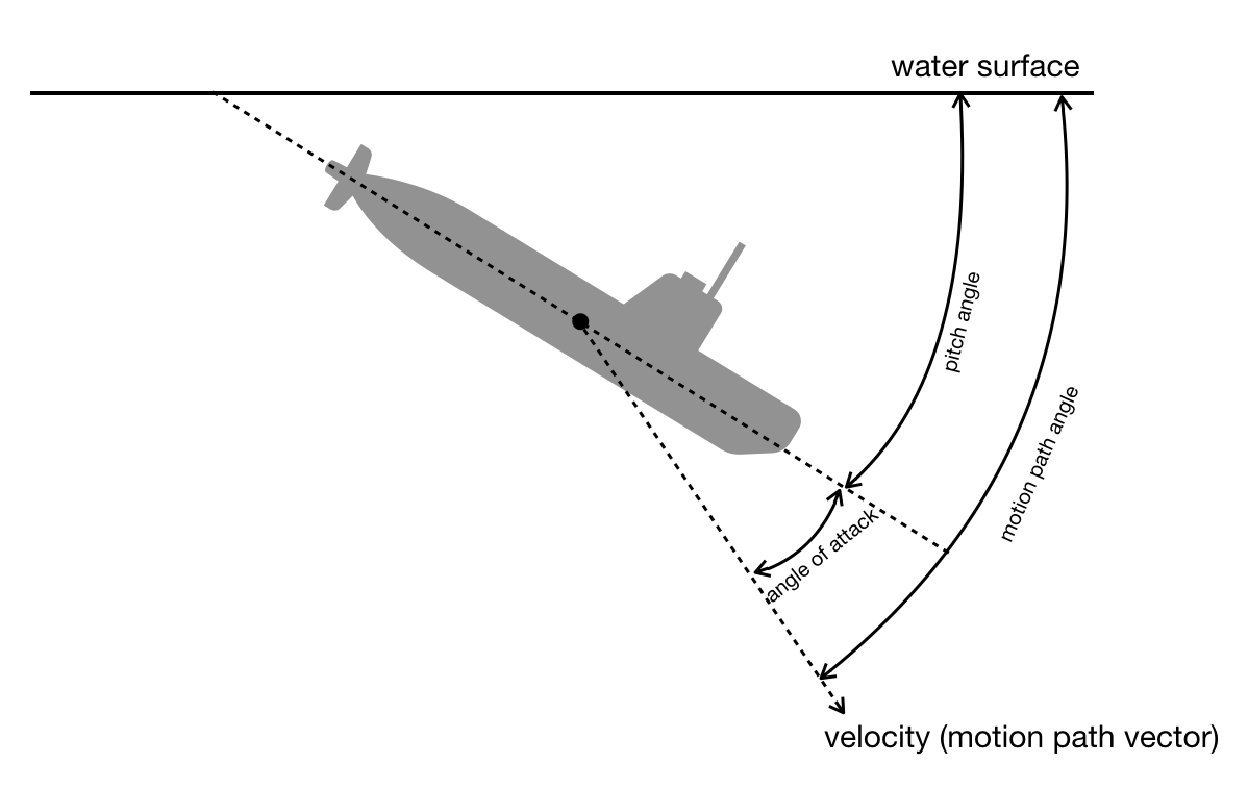
\includegraphics[width=0.85\textwidth]{PathAngle.eps}
\caption{Trajectory angles}	
\label{FIG:PathAngle}
\end{figure}
\section{Frenet-Serret Frame}
The underwater robots have six dynamic variables (3 linear velocities and 3 angular velocities) and six kinematic variables (positions and Euler angles in inertial frame $\lbrace i \rbrace$), all of which fully describes the robot's behaviour together. The trim trajectory merely offer us the information about the desired kinematic position, we still lack the data about the desired orientation (Euler angles) and the desired velocities along these trim trajectories. The Frenet-Serret model has the advantage of being a well-established means of modeling continuous spatial curves. The definition of the Frenet-Serret frame is elaborated in follows: 

When a particle moves along a continuous, differentiable curve in three-dimensional Euclidean space $\mathbb{R}^{3}$, its motion can be characterized by three unit vectors: $\vec{T}^{i}(t)$, $\vec{N}^{i}(t)$ and $\vec{B}^{i}(t)$. $\vec{T}^{i}(t)$ is a unit vector tangent to the curve, denoting the motion direction. 
\begin{align}
\vec{T}^{i}(t)=\dfrac{\vec{\eta}_{\mathcal{T}}^{'}(t)}{||\vec{\eta}_{\mathcal{T}}^{'}(t)||}.
\end{align}    
The normal vector $\vec{N}^{i}(t)$ is equal to the derivative with respect to the arclength parameter of the curve divided by its length which can be calculated as follows:
\begin{align}
\vec{N}^{i}(t)=\dfrac{\vec{T}^{'}(t)}{||\vec{T}^{'}(t)||}=
\dfrac{\vec{\eta}_{\mathcal{T}}^{'}(t)\times (\vec{\eta}_{\mathcal{T}}^{''}(t)\times \vec{\eta}_{\mathcal{T}}^{'}(t))}{||\vec{\eta}_{\mathcal{T}}^{'}(t)||\cdot||\vec{\eta}_{\mathcal{T}}^{''}(t)\times \vec{\eta}_{\mathcal{T}}^{'}(t))||}.
\end{align}
The binomal vector $\vec{B}^{i}(t)$ is the cross product of the normal vector $\vec{N}^{i}(t)$ and the tangent vector $\vec{T}^{i}(t)$ and is calculated as 
\begin{align}
\vec{B}^{i}(t)=\vec{T}^{i}(t) \times \vec{N}^{i}(t)=
\dfrac{\vec{\eta}_{\mathcal{T}}^{''}(t)\times \vec{\eta}_{\mathcal{T}}^{'}(t)}{||\vec{\eta}_{\mathcal{T}}^{''}(t)\times \vec{\eta}_{\mathcal{T}}^{'}(t))||}.
\end{align}
These three vectors are expressed in inertial world frame $\left\lbrace i \right\rbrace$ because they describe the kinematic property of the robot. $\vec{T}^{i}(t)$, $\vec{N}^{i}(t)$ and $\vec{B}^{i}(t)$ constitute an orthonormal basis spanning in $\mathbb{R}^{3}$ and we use $\left\lbrace FS\right\rbrace$ to denote the Frenet-Serret frame.

The transformation matrix from the Frenet-Serret frame to the inertial world frame $\lbrace i \rbrace$ is defined as
\begin{align}
 \emph{\textbf{R}}_{FS}^{i} &=
 (\vec{T}^{i}(t) \quad \vec{N}^{i}(t) \quad \vec{B}^{i}(t)) \nonumber \\
 &=
 \begin{pmatrix}
c\psi_{\mathcal{T}} c\theta_{\mathcal{T}}&-s\psi_{\mathcal{T}} c\phi_{d}+c\psi_{\mathcal{T}} s\theta_{\mathcal{T}} s\phi_{\mathcal{T}}&s\psi_{\mathcal{T}} s\phi_{\mathcal{T}}+c\psi_{\mathcal{T}} c\phi_{\mathcal{T}} s\theta_{\mathcal{T}} \\
s\psi_{\mathcal{T}} c\theta_{\mathcal{T}}&c\psi_{\mathcal{T}} c\phi_{\mathcal{T}}+s\phi_{\mathcal{T}} s\theta_{\mathcal{T}} s\psi_{\mathcal{T}}&-c\psi_{\mathcal{T}} c\phi_{\mathcal{T}}+s\theta_{\mathcal{T}} s\psi_{\mathcal{T}} c\phi_{\mathcal{T}}\\
-s\theta_{\mathcal{T}}&c \theta_{\mathcal{T}} s \phi_{\mathcal{T}}&c \theta_{\mathcal{T}} c\phi_{\mathcal{T}}
\end{pmatrix}
\end{align}
Thus, we can calculate the desired orientation (Euler angles) $\vec{\lambda}_{\mathcal{T}}=(\phi_{\mathcal{T}},~\theta_{\mathcal{T}},
~\psi_{\mathcal{T}})^{T}$ along the trim trajectory as follows:
\begin{align}
\theta_{\mathcal{T}}=-\sin^{-1}(\vec{T}^{i}(t)),
\end{align}
\begin{align}
\phi_{\mathcal{T}}=-\sin^{-1}(\sec(\theta_{\mathcal{T}})\cdot \vec{N}^{i}(t))
\end{align}
The desired yaw angle comes from the definition of the trim trajectory:
\begin{align}
\psi_{\mathcal{T}}=\dot{\psi}_{\mathcal{T}}t+\psi_{0}.
\end{align}
In the previous discussions, we have derived the complete desired kinematic states $\vec{\eta}_{\mathcal{T}}=(\vec{p}_{\mathcal{T}},~\vec{\lambda}_{\mathcal{T}})^{T}$ for underwater robots for the trim trajectory. The desired dynamic states can be determined 
from the kinematics with help of the rotation  matrix $ \emph{\textbf{R}}_{FS}^{i}$.

For a given trim trajectory, we can calculate the desired velocities as follows:
\begin{align}
\vec{\upsilon}_{\mathcal{T}}=
\begin{pmatrix}
\vec{v}_{\mathcal{T}} \\
\vec{\omega}_{\mathcal{T}}
\end{pmatrix}=
(\emph{\textbf{R}}_{FS}^{i})^{-1}.
\end{align}

In conclusion, the 12 state variables $\vec{x}_{\mathcal{T}}=(\vec{\eta}_{\mathcal{T}}$,~$\vec{\upsilon}_{\mathcal{T}})^{T}$ fully specify the kinematics and dynamics the robot should perform along the trim trajectory. We will use the desired states to derive the error dynamics in the next chapter.


